\minitoc
\begin{refsection}
\newpage
\fbox{\begin{minipage}{\textwidth}
    \textbf{Contexte :}\\
    En dépit de son importance fondamentale en électrodynamique quantique et en astrophysique des hautes énergies, le processus de création de paires électron-positron par collision de deux photons réels, appelé processus Breit-Wheeler linéaire, n'a jusqu'à présent jamais été observé directement en laboratoire depuis sa prédiction en 1934. Cette expérience nécessiterait de pouvoir produire des sources de photons dans la gamme du MeV.
    
    \medskip
    \textbf{Résumé du chapitre :}\\
    Dans ce chapitre, la place du processus Breit-Wheeler linéaire est contextualisée dans le cadre de l'électrodynamique quantique, et ses liens avec des processus théoriquement très proches sont explicités (figure \ref{fig:1-diagrammes_electron-positron}). Parmi ces autres processus de création de paires, des estimations permettent de montrer que la création de paires par absorption d'un photon au voisinage d'une charge électrique (processus Bethe-Heitler et Triplet) pourra éventuellement constituer un bruit de mesure pour les conditions expérimentales considérées dans la suite de ce manuscrit. Des processus permettant de produire des photons dans la gamme du MeV, tel que les processus Compton inverse linéaire, Compton inverse multi-photon et Bremsstrahlung, sont ensuite abordés (figure \ref{fig:12-diagrammes_gamma}). Ce chapitre se termine par une présentation des principaux processus ayant lieu lors de la propagation d'électrons ou de photons dans la matière (figure \ref{fig:12-processus_matiere}).
    
    \medskip
    \textbf{Informations complémentaires :}\\
    Une introduction au cadre théorique de l'électrodynamique quantique est disponible en référence \parencite{klauber_2015}, dont le premier chapitre offre un rapide survol du domaine. Les aspects plus conceptuels et philosophiques sont discutés dans l'ouvrage \parencite{teller_1997} qui est à la fois court et clair, et les aspects techniques liés au calcul de sections efficaces (en particulier de la section efficace Breit-Wheeler linéaire) sont développés notamment dans \parencite{greiner_2009}. Les principaux mécanismes ayant lieu lors de la propagation de particules énergétiques dans la matière sont quant à eux présentés dans le très synthétique ouvrage \parencite{carron_2007}.
\end{minipage}}
\newpage

\section{Collision de particules}
Cette section présente rapidement le cadre théorique nécessaire à la description du processus Breit-Wheeler linéaire. Ce dernier doit être décrit par une théorie à la fois relativiste et quantique, permettant la création de paires électron-positron, tel que l'électrodynamique quantique. La proximité de ce processus avec d'autres processus de création de paires sera évoqué, notamment avec ceux faisant intervenir des photons dits virtuels. 

\subsection{Contexte général}

Dans le cadre de cette thèse, nous nous intéresserons aux processus de collision de photons, et plus particulièrement au processus de \textbf{création de paires électron-positron par collision de deux photons réels}. Ce mécanisme de création de paires de leptons, nommé \textbf{Breit-Wheeler linéaire} (noté \textit{BWL} dans la suite du manuscrit) en l'honneur de G. Breit et J. A. Wheeler qui furent les premiers à l'étudier théoriquement en 1934 \parencite{breit_1934}, ne peut être compris que d'un point de vue \textbf{quantique}, dans le sens qu'il fait intervenir les quanta du champ électromagnétique : des photons. Le cadre théorique nécessaire à la description de ce processus doit alors prendre en compte la nature quantique de l'interaction, mais aussi permettre la modification du \textbf{nombre} et du \textbf{type de particules} en présence entre l'état initial et l'état final du processus, et doit être compatible avec les postulats de la \textbf{relativité restreinte}, puisque les électrons, positrons et photons peuvent se mouvoir à des vitesses proches de la vitesse de la lumière dans le vide (notée ici $c$).

La théorie de l'\textbf{électromagnétisme} synthétisée par les équations de Maxwell permet d'étudier l'évolution de champs électromagnétiques, mais n'est pas quantique. Un de ses principe fondamentaux est le \textbf{principe de superposition}, qui implique que l'amplitude de deux ondes électromagnétiques se propageant en un même point s'ajoutent simplement, sans pouvoir interagir. L'interaction entre ondes dans le vide (ou entre photons dans le langage des particules) n'est donc pas possible dans ce cadre théorique. La prise en compte des principes de la relativité restreinte dans l'interaction ondes-particules est synthétisée dans le cadre théorique de l'électrodynamique classique, qui sera le cadre privilégié de la suite de cette thèse. 

La \textbf{mécanique quantique non relativiste} traite quant à elle de l'état de particules, et permet notamment de calculer l'évolution de leur fonction d'onde via l'équation de Schrödinger. Ce cadre théorique permet de décrire l'évolution conjointe de plusieurs particules, mais la \textbf{modification} de leur \textbf{nombre} et de leur \textbf{type} n'y est en général \textbf{pas possible} pour des particules non composites (e.g. il est possible de décrire l'ionisation d'un atome d'hydrogène évoluant en un électron et un proton libres, mais pas l'annihilation d'une paire électron-positron en une paire de muons) \parencite{klauber_2015}. La prise en compte des effets relativistes permet de décrire les particules de spin nul via l'équation de Klein-Gordon, les particules de spin $1/2$ via l'équation de Dirac, et les particules de spin $1$ via l'équation de Proça \parencite{klauber_2015}.

Pour décrire des systèmes où \textbf{le nombre et le type de particules} peuvent \textbf{évoluer avec le temps}, il est usuellement nécessaire d'utiliser le cadre théorique de la \textbf{théorie quantique des champs}. En particulier, la théorie quantique des champs traitant de l'interaction électromagnétique est appelée électrodynamique quantique, et sera notée \textit{QED} (pour \textit{Quantum Electrodynamics}). Cette dernière ne prend en compte ni les interactions faible, forte ou gravitationnelle, mais est à l'heure actuelle la théorie physique la mieux vérifiée expérimentalement, avec des prédictions correctes jusqu'à plus de la neuvième décimale dans certains domaines (par exemple pour la prédiction du moment anomal de l'électron \parencite{klauber_2015}). L'application de ses prédictions à l'échelle cosmologique pose néanmoins des problèmes majeurs (avec une énergie du vide de 120 ordres de grandeur supérieure à celle qui serait attendue pour expliquer la constante cosmologique \parencite{weinberg_1989}), et la conciliation entre le formalisme de la théorie quantique des champs (comprenant l'électrodynamique quantique mais pas seulement) et celui de la relativité générale est encore un problème ouvert aujourd'hui en physique théorique \parencite{klauber_2015, kuhlmann_2018}. D'un point de vue fondamental, des développements sont aussi en cours pour tenter de dériver son formalisme à partir d'une axiomatique bien définie \parencite{kuhlmann_2018}, et certains de ses aspects se heurtent à des problèmes d'interprétations (e.g. la présence de valeurs de charge et de masse infinies, qui pourrait indiquer que cette théorie est seulement valide aux plus "basses" énergies \parencite{kuhlmann_2018, teller_1997}). L'étude de ses prédictions en présence d'un fort champ électromagnétique présente aussi un intérêt théorique important \parencite{dipiazza_2012, dunne_2009}, et les lasers de haute puissance en cours de construction permettront a priori d'étudier expérimentalement certaines de ces prédictions dans des régimes non-linéaires \parencite{dipiazza_2012}, voire non-perturbatifs \parencite{dipiazza_2012, dunne_2009} (plus de détails sur les lasers de haute puissance seront donnés au chapitre \ref{chap:2-laser}). Certains points communs et différences entre ces divers cadres théoriques sont illustrés dans le tableau \ref{fig:21-tableau_comparaison_theories}.

\begin{figure}[hbtp]
	\centering
	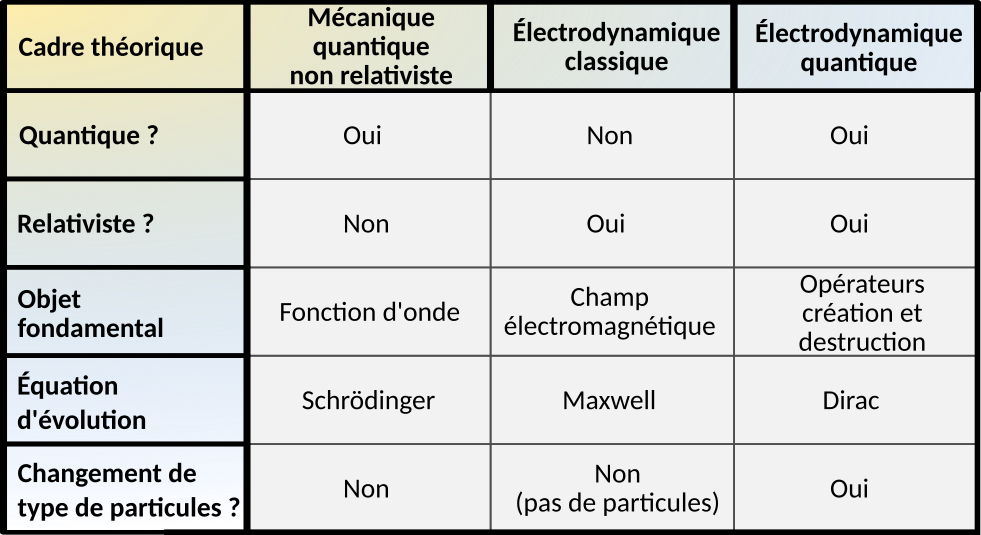
\includegraphics[width=\linewidth]{1-particules/tableau_comparaison_theories.png}
	\caption{Comparaison de différents cadres théoriques permettant la description de particules ou d'ondes électromagnétiques. Inspiré de \parencite{klauber_2015}.}
	\label{fig:21-tableau_comparaison_theories}
\end{figure}

La discussion plus approfondie de ces aspects dépasse néanmoins largement le cadre de cette thèse, et le processus BWL auquel nous allons nous intéresser fait partie des plus simples de l'électrodynamique quantique d'un point de vue théorique. Celui-ci est représenté en figure \ref{fig:1-diagrammes_electron-positron}a.

\begin{figure}[hbtp]
	\centering
	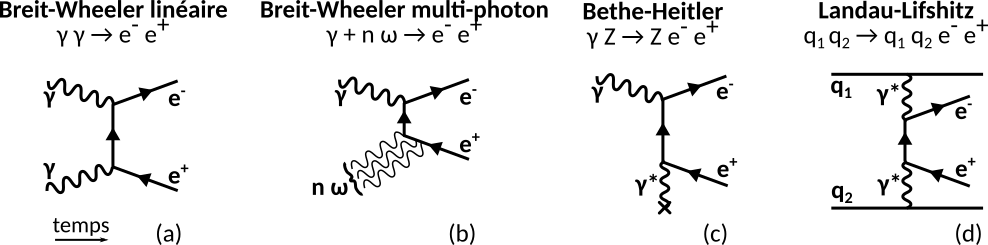
\includegraphics[width=\linewidth]{1-particules/QED_electron-positron.png}
	\caption{Exemples de diagrammes de Feynman, pour des processus de création de paires par collision de photons. Le symbole $\gamma$ correspond à un photon réel dans le vide, $e^-$ et $e^+$ respectivement à un électron et un positron, $n \omega$ à un nombre entier de photons laser, $\gamma^*$ à un photon virtuel, $Z$ à un noyau d'atome et $q_1$, $q_2$ à des particules chargées électriquement.}
	\label{fig:1-diagrammes_electron-positron}
\end{figure}

Sur cette figure, les lignes ondulées représentent des photons et lignes droites des électrons ou positrons. Le temps est représenté horizontalement et est croissant de gauche à droite, et l'espace est représenté par une seule dimension dans la direction verticale. Sur ce diagramme temps-espace, deux photons arrivent donc de la gauche (de $t \to - \infty$), alors que deux lignes représentant un électron et un positron quittent le diagramme par la droite (vers $t \to + \infty$). Par convention, on désigne les particules (ici l'électron) par des flèches dans le sens du temps, et des anti-particules (ici le positron) dans le sens inverse du temps. Ce diagramme indique donc que deux photons entrent dans la zone de collision et qu'une paire électron-positron en ressort, et fait donc bien référence au processus Breit-Wheeler linéaire. 

En plus de permettre une visualisation pratique de différents processus, les diagrammes du type de ceux représentés en figure \ref{fig:1-diagrammes_electron-positron} peuvent aussi être un moyen de calculer quantitativement les probabilités de transition de l'état initial (à gauche) à l'état final (à droite). Ceux-ci sont alors appelés diagrammes de Feynman, et cette probabilité de transition est calculée à partir d'une superposition de diagrammes, qui représentent chacun un terme d'un développement perturbatif (ces règles de calcul ne seront néanmoins pas détaillées ici, mais peuvent être retrouvées notamment dans les références \parencite{klauber_2015} et \parencite{greiner_2009}). En pratique, la \textbf{probabilité de transition} entre l'état initial et final du processus est souvent formalisée par une quantité nommée \textbf{section efficace}, qui est \textbf{homogène à une surface}, et est souvent notée $\sigma$. La description de ces processus par l'intermédiaire de ce type de diagramme fait donc à la fois intervenir des lignes représentant les particules incidentes et les particules produites (qui peuvent éventuellement être identiques dans le cas d'une diffusion), appelées \textit{particules réelles}, mais contiens aussi des \textbf{lignes internes} qui sont souvent associées à des "particules" appelées \textit{particules virtuelles} \parencite{jaeger_2019}. Celles-ci ne sont donc, par définition, pas directement mesurables, mais produisent tout de même des effets qui, eux, sont mesurables \parencite{jaeger_2019}. Ces particules modélisent l'interaction entre particules réelles ou virtuelles, mais ne présentent néanmoins pas les propriétés habituelles attendues pour des particules, comme pouvoir être localisées et comptées \parencite{teller_1997}, et ne satisfont pas en général à la relation énergie-impulsion $E^2 = p^2 c^2 + m^2 c^4$ (elles sont alors dites "hors couche de masse" \parencite{jaeger_2019}). Une analogie ondulatoire permet aussi de les associer à une onde évanescente ou à une oscillation forcée, alors que les particules réelles sont associées à une onde plane \parencite{lawson_1970}. Les interprétations à donner aux termes "particules réelle" et "particule virtuelle" sont néanmoins toujours aujourd'hui l'objet de discussions et de débats en philosophie des sciences \parencite{teller_1997, kuhlmann_2018, marburger_1996, jaeger_2019}.

Dans le cadre de l'électrodynamique quantique, le champ électrostatique émis par une charge électrique peut donc être décrit par l'intermédiaire d'un photon virtuel. Ainsi, la création de paires électron-positron par un photon réel au voisinage d'un noyau d'atome, représenté en figure \ref{fig:1-diagrammes_electron-positron}c et appelé processus \textit{Bethe-Heitler}, peut alors être interprétée comme étant la conséquence de la création de paires par \textbf{collision d'un photon réel avec un photon virtuel}. De la même manière, la création de paires dans la diffusion de particules chargées, représenté en figure \ref{fig:1-diagrammes_electron-positron}d et appelé processus \textit{Landau-Lifshitz}, peut être interprété comme étant la conséquence de la création de paires par \textbf{collision de deux photons virtuels}. Pour le calcul des probabilités de transitions, ces photons virtuels sont parfois assimilés à des photons réels si leur \textit{coefficient de virtualité}, défini par $Q^2=E^2-p^2c^2$, est proche de $Q^2 \sim 0$ \parencite{greiner_2009} (ceux-ci sont alors généralement appelés \textit{quasi-réels}). Sous ces conditions, la probabilité de création de paires par collision de photons virtuels est supposée identique à la probabilité de création de paires par collision de photons réels, calculée à partir du diagramme \ref{fig:1-diagrammes_electron-positron}. Autrement dit, le calcul de la section efficace du processus Landau-Lifshitz fait intervenir la section efficace Breit-Wheeler linéaire. Cette hypothèse porte le nom d'\textbf{approximation de photon équivalent} \parencite{greiner_2009, kessler_1974}, et a été très largement étudiée depuis les années 70 dans les collisionneur de particules \parencite{budnev_1975}, mais garde toujours un très grand intérêt aujourd'hui \parencite{klein_2020, starcollaboration_2019}. Ainsi, la détection de positrons produits par absorption d'un photon réel au voisinage d'un noyau d'atome, ou produits dans la collision de particules chargées constitue, d'un point de vue théorique, une mesure \textit{indirecte} du processus de création de paires par collision de photons réels BWL. Ces deux processus ont déjà été largement observés et étudiés par propagation de particules dans la matière \parencite{hubbell_2006} et dans les collisionneurs de particules \parencite{budnev_1975}, où les premières mesures remontent respectivement aux années 1930 \parencite{anderson_1933} et 1970 \parencite{balakin_1971}. De plus, la détection de la \textbf{création de paires par interaction d'un photon de plusieurs dizaines de giga-électronvolts (GeV) avec un laser} a quant à elle été détectée en 1997 \parencite{burke_1997}, et est interprété dans le cadre de l'électrodynamique quantique en champ fort comme la collision d'\textbf{un photon de haute énergie} avec \textbf{plusieurs photons de basse énergie}. Ce processus, représenté en figure \ref{fig:1-diagrammes_electron-positron}b, y est alors appelé processus Breit-Wheeler \textbf{multi-photon} (les termes "non-linéaire" et "multi-photon" seront dans ce contexte utilisés de manière interchangeables \parencite{greiner_2009}). Enfin, le processus d'annihilation électron-positron en deux photons a lui aussi pu être observé dès 1934 \parencite{klemperer_1934}, et correspond au symétrique du processus Breit-Wheeler linéaire par renversement du temps.

Dans un contexte astrophysique, le processus BWL est aussi supposé jouer un rôle important dans l'opacité de l'Univers aux photons de très hautes énergies, car ceux-ci pourraient produire des paires $e^-e^+$ en collisionnant avec des photons émis par divers objets, comme des photons optiques émis par des étoiles, ou du rayonnement radio émis par des galaxies, voire même avec le fond diffus cosmologique pour des photons d'énergie de l'ordre la centaine de TeV \parencite{diehl_2001, nikishov_1961, gould_1967a}. Ce processus pourrait aussi être à l'origine de jets de paires au voisinage de trous noirs supermassifs \parencite{bonometto_1971} ou de pulsars \parencite{zhang_1998}.

Ainsi, et comme le font remarquer les auteurs \cite{gould_1967}, étant donnée la remarquable précision des prédictions de l'électrodynamique quantique et l'observation directe de processus théoriquement très proches (annihilation électron-positron, processus Breit-Wheeler multi-photon, création de paires par collision de photons virtuels), l'existence en tant que telle du processus Breit-Wheeler linéaire est fortement probable ("ne peux pas être questionnée" selon eux). Néanmoins, son observation directe en laboratoire reste aujourd'hui toujours à être démontrée car, comme le notaient déjà G. Breit et J. A. Wheeler dans leur article de 1934 \parencite{breit_1934}, ce processus est difficilement mesurable expérimentalement à cause de la faible valeur de sa section efficace, et surtout des faibles flux de photons d'énergies autour du $\si{\MeV}$ disponibles en laboratoire à cette époque. Nous verrons néanmoins aux chapitres \ref{chap:2-laser} et \ref{chap:3-methodes_exp} que le développement des lasers intenses permet d'envisager de mener cette expérience sur des installations existantes ou en cours de construction, et que plusieurs équipes travaillent actuellement à ce sujet. D'un point de vue plus général, la thématique de la collision de photons réels est elle aussi très actuelle \parencite{marklund_2006, chou_2018, takahashi_2019}, ainsi que l'utilisation de lasers pour mener de nouvelles études d'électrodynamique quantique \parencite{dipiazza_2012, zhang_2020}. 

\subsection{Création de paires électron-positron par collision de photons}

Dans le cadre de cette thèse, nous serons donc particulièrement intéressés par la création de paires de leptons chargés via la collision de photons réels, et en particulier par la création de paires électron-positron, car ceux-ci sont de plus faible masse et donc plus simples à produire en laboratoire. Les résultats développés dans la suite de ce manuscrit pourraient néanmoins être réadaptés à la création de paires de leptons plus massifs, tels que les muons par exemple, qui ont une masse $\sim 200$ fois supérieure à celle des électrons et positrons.

Dans la suite de cette section, les deux photons incidents du processus BWL seront notés $1$ et $2$, et toutes les quantités y faisant référence auront un indice $1$ ou $2$, ou un indice $i$ lorsque la définition vaut pour les deux photons. Les quantités faisant référence aux électrons et aux positrons seront désignées par un indice respectivement $-$ et $+$, ou par un indice $e$ lorsque la définition vaut pour les deux types de particules. Le référentiel du laboratoire sera noté $\mathcal{R}$ et les quantités exprimées dans ce référentiel n'auront aucun exposant, alors que le référentiel du centre d'inertie du système de particules sera noté $\mathcal{R}^*$ et toutes les quantités exprimées dans ce référentiel auront un exposant $*$. L'énergie totale du système de particules exprimée dans le centre d'inertie (appelée par la suite "énergie du centre d'inertie") pourra néanmoins être notée sans exposant $*$ car celle-ci est invariante de Lorentz. Le centre d'inertie, ou centre des impulsions, sera aussi noté \textit{CM} pour \textit{center of momentum}, et afin de ne pas confondre l'acronyme "CI" avec le processus Compton inverse qui sera discuté dans la section suivante. Les quadri-vecteurs seront notés par des lettres majuscules et soulignés $\underline{X}$ et les vecteurs dans l'espace tridimensionnel seront notés en lettres minuscules avec une flèche $\vec{x}$. La norme des vecteurs sera indiquée par le même symbole sans flèche $x$. On se placera aussi dans le système d'unités naturelles, où la vitesse de la lumière vaut $c=1$. Dans ce cas, l'énergie, l'impulsion et la masse ont la même unité, et seront généralement exprimés en méga-électronvolts ($\si{\MeV}$).

\subsubsection{Création de paires électron-positron par collision de deux photons réels}

Dans tout processus de collision de particules, la somme des énergies des particules incidentes (énergies cinétiques et énergies de masse) doit égaler la somme des énergies des particules produites (énergies cinétiques et énergies de masse), par conservation de l'énergie. Pour le processus de création de paires électron-positron par collision de deux photons réels, la masse des particules incidentes (les photons) est nulle, alors que celle des particules produites est non nulle, de valeur identique pour les électrons et les positrons, et notée $m_e$. Ainsi, le processus BWL est un \textbf{processus à seuil} en énergie, puisque la somme de l'énergie des photons incidents devra au minimum égaler l'énergie de masse des particules produites, soit $2 m_e c^2$ (noté simplement $2 m_e$ dans la suite, puisque dans le système d'unités naturelles $c=1$). Pour deux photons incidents d'énergie $m_e$, la création de paires électron-positron (notés par la suite respectivement $e^-$ et $e^+$) n'est en fait possible que si l'énergie des photons réels incidents (notés $\gamma$ dans la suite) est rigoureusement identique, et qu'ils collisionnent avec un angle de 180 degrés. Dans ce cas, les paires $e^- e^+$ sont créées au repos dans le référentiel du laboratoire.

D'un point de vue plus général, la \textbf{condition de création de paires} nécessite que l'\textbf{énergie totale dans le centre d'inertie dépasse l'énergie de masse des particules produites}, soit $2 m_e$. Le carré de l'énergie totale disponible dans le centre d'inertie de la collision peut être calculé comme étant :
\begin{equation}
    s = (\underline{P}_1+\underline{P}_2)^2 = E_{CM}^2 ~ \rm ,
    \label{eq:1-s_definition}
\end{equation}
où $s$ est la variable de Mandelstam de masse invariante, qui est un invariant relativiste, où $E_{CM}$ est l'énergie totale dans le centre d'inertie de la collision, et où $\underline{P}_i=(E_i, \vec{p}_i)$ est la quadri-impulsion du photon incident $i$, avec $E_i$ son énergie, $\vec{p}_i$ son impulsion, et avec $i=\{1,2\}$. En choisissant un repère cartésien tel que le plan $(x,z)$ coïncide avec le plan de collision des photons, et où l'axe $z$ est colinéaire à la bissectrice des photons, l'impulsion des photons peut s'écrire $\vec{p}_1= - p_1 \sin(\psi_{12}/2) \vec{e}_x + p_1 \cos(\psi_{12}/2) \vec{e}_z$ et $\vec{p}_2=p_2 \sin(\psi_{12}/2) \vec{e}_x + p_2 \cos(\psi_{12}/2) \vec{e}_z$, où $p_i$ est la norme de $\vec{p}_i$, $\psi_{12}$ est l'angle de collision entre les photons et où $\vec{e}_x$, $\vec{e}_z$ sont les vecteurs de base dans les directions $x$ et $z$ positives. Ce repère est illustré en figure \ref{fig:1-repere_cinematique}a. Dans ce cas, en considérant une métrique de Minkowski $(+,-,-,-)$, l'équation (\ref{eq:1-s_definition}) peut s'écrire :
\begin{equation}
    s = \underline{P}_1^2+\underline{P}_2^2+2\underline{P}_1\cdot\underline{P}_2 = (E_1^2-p_1^2)+(E_2^2-p_2^2)+2\left(E_1 E_2-p_1 p_2 \left[-\sin^2(\psi_{12}/2)+\cos^2(\psi_{12}/2)\right]\right) ~ \rm .
\end{equation}

En sachant que $\cos^2(x/2)-\sin^2(x/2)=\cos(x)$, et que pour des photons $E_i^2=p_i^2$, on a donc finalement :
\begin{equation}
    s=2 E_1 E_2 (1-\cos{\psi_{12}})=E_{CM}^2 ~ \rm .
\end{equation}

La condition (nécessaire mais pas suffisante) de création de paires peut donc simplement s'écrire $\sqrt{s} \ge 2 m_e$. En utilisant le formalisme de l'électrodynamique quantique, il est aussi possible de calculer la \textbf{probabilité} de création de paires électron-positron par collision de photons, qui est usuellement modélisée par une \textbf{section efficace}, notée $\sigma_{\gamma\gamma\to e^-e^+}$ ou plus simplement $\sigma_{\gamma\gamma}$, et qui vaut ici \parencite{greiner_2009} : 
\begin{equation}
    \sigma_{\gamma\gamma\to e^-e^+} (s) =4 \pi r_e^2 \frac{m_e^2}{s} \left[ \left(2 + \frac{8 m_e^2}{s} - \frac{16 m_e^4}{s^2}\right) \ln \frac{\sqrt{s} + \sqrt{s - 4 m_e^2}}{2 m_e} - \sqrt{1 - \frac{4 m_e^2}{s}}\left(1 + 4 \frac{m_e^2}{s}\right)\right] ~ \rm ,
    \label{eq:1-sigma_BWL}
\end{equation}
où $r_e = e^2/4 \pi \varepsilon_0  m_e c^2 \approx 2.8 \times 10^{-13} ~ \si{\cm}$ est le rayon classique de l'électron. Dans le cadre de cette thèse, nous nous limiterons à l'utilisation de la section efficace totale non polarisée $\sigma_{\gamma\gamma}$, et ne prendront en compte ni l'effet de la section efficace différentielle en angle solide, ni l'effet de la polarisation des photons ou encore l'effet d'un champ électromagnétique externe. Plus d'informations sont néanmoins disponibles sur ces aspects respectivement dans les références \parencite{ribeyre_2018}, \parencite{yasui_1993} et \parencite{hartin_2007, satunin_2018}, notamment.

Cette \textbf{section efficace totale dépend uniquement} de la variable de Mandelstam $s$, ou de manière équivalente \textbf{de l'énergie totale dans le centre d'inertie}. Elle est tracée en fonction de l'énergie des photons incidents considérées égales $E_1=E_2$ et pour différents angles de collision $\psi_{12}$ en figure \ref{fig:1-sigma_BWL}a, ou en fonction de $\sqrt{s}=E_{CM}$ en figure \ref{fig:1-sigma_BWL}b. L'effet de seuil de création de paires y est bien représenté pour $\sqrt{s}\ge 2 m_e \approx 1.02 ~ \si{\MeV}$, et elle atteint un maximum de l'ordre de  $2.1 \times r_e^2 \approx 1.6 \times 10^{-25} ~ \si{\cm^2}$ pour une valeur de $\sqrt{s}$ autour de $1.43 ~ \si{\MeV}$. Pour des photons de même énergie collisionnant avec un angle $\psi_{12}$, la probabilité de création de paires est donc maximisée pour une énergie des photons incidents de l'ordre de $1 \si{[\MeV]}/\sqrt{1-\cos{\psi_{12}}}$. La valeur de la section efficace est divisée par $10$ par rapport à sa valeur maximale pour $\sqrt{s} \approx 8.47 ~ \si{\MeV}$. Il est intéressant de noter que $\sigma_{\gamma\gamma}$ ne dépend pas directement de l'énergie de chaque des photons incidents, mais dépend uniquement du \textbf{produit de leur énergie}. Ainsi, le \textbf{seuil de création de paires} peut être atteint pour des énergies de photons incidents très variées, comme par exemple dans la collision de \textbf{deux photons d'énergie dans la gamme du MeV}, mais aussi pour un photon de \textbf{quelques centaines de MeV} collisionnant avec un photon d'énergie autour de \textbf{quelques keV}, ou encore pour un photon dans la \textbf{gamme du GeV} collisionnant avec un photon de \textbf{quelques centaines d'eV} ; en supposant un angle de collision de $180$ degrés. La \textbf{diminution de l'angle de collision} a pour effet d'\textbf{augmenter l'énergie minimale des photons nécessaire permettant d'atteindre le seuil de création de paires}.

\begin{figure}[hbtp]
	\centering
	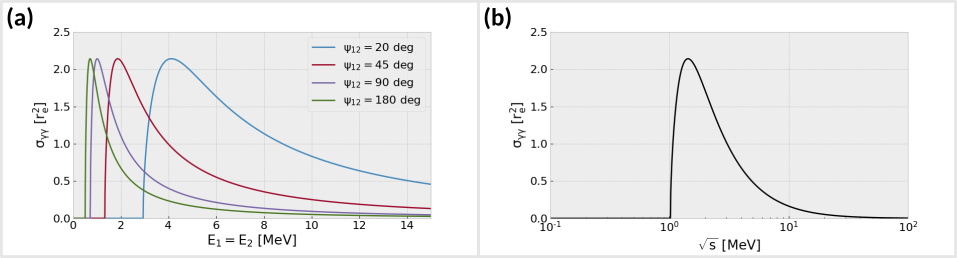
\includegraphics[width=\linewidth]{1-particules/sigma_BWL.png}
	\caption{Section efficace totale du processus Breit-Wheeler linéaire, exprimée en $r_e^2$, (a) en fonction de l'énergie des photons incidents, supposées égales, exprimées en $\si{\MeV}$, et pour différents angles de collision, ou (b) en fonction de l'énergie du centre d'inertie $\sqrt{s}$ exprimée en $\si{\MeV}$.}
	\label{fig:1-sigma_BWL}
\end{figure}

Pour déterminer la direction de propagation des électrons et positrons produits, il est généralement plus simple de commencer par se placer \textbf{dans le référentiel du centre d'inertie de la collision}, noté $\mathcal{R}^*$ et illustré en figure \ref{fig:1-repere_cinematique}b. En effet, dans ce repère la \textbf{somme des impulsions des photons} incidents est \textbf{nulle}, par définition du centre d'inertie. Ainsi, la somme des impulsions des particules émises doit elle aussi y être nulle, par conservation de l'impulsion. Lors de la création d'une paire électron-positron, \textbf{l'impulsion de l'électron et du positron} produits sont donc strictement \textbf{identiques en norme}, et \textbf{opposées en direction}. Dans ce cas, les \textbf{énergies totales de l'électron et du positron} sont aussi \textbf{identiques}, et valent respectivement $E_-^*=E_+^*=E_{CM}/2$ . En première approximation, il est possible de considérer que la \textbf{direction d'émission} des particules est \textbf{isotrope} dans le référentiel du centre d'inertie \parencite{ribeyre_2017}. L'effet de la section efficace différentielle est étudié dans la référence \parencite{ribeyre_2018}, et l'émission des paires dans $\mathcal{R}^*$ commence à exhiber deux directions privilégiées pour $\sqrt{s} \gtrsim 1.5 ~ \si{\MeV}$.

\begin{figure}[hbtp]
	\centering
	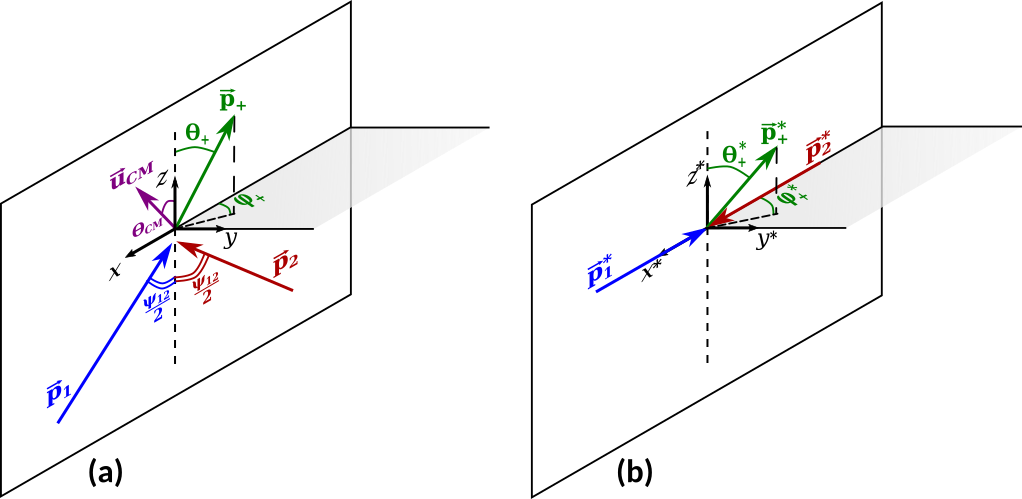
\includegraphics[width=\linewidth]{1-particules/basis_definition.png}
	\caption{Définition des repères et quantités pour la création de paires par collision de photons, où (a) est le repère du laboratoire $\mathcal{R}$ et où (b) est le repère du centre d'inertie $\mathcal{R}^*$.}
	\label{fig:1-repere_cinematique}
\end{figure}

Si le référentiel du laboratoire $\mathcal{R}$ et le référentiel du centre d'inertie $\mathcal{R}^*$ ne sont pas superposés (i.e. si $\vec{p}_1+\vec{p}_2 \neq \vec{0}$ dans le référentiel du laboratoire), alors l'impulsion et l'énergie des particules produites est \textbf{modifiée lors d'un changement de référentiel}. Dans le cas général, l'impulsion et l'énergie d'un positron (ou de manière équivalente d'un électron) dans le référentiel du laboratoire, notés respectivement $\vec{p}_+$ et $E_+$, peuvent alors être calculées via une transformation de Lorentz appropriée \parencite{ribeyre_2017, furry_1955} :
\begin{equation}
\begin{split}
    \vec{p}_+   &= \vec{p}_+^* + \dfrac{(\gamma_{CM} - 1)}{\beta_{CM}^2} (\vec{\beta}_{CM} \cdot \vec{p}_+^*) ~ \vec{\beta}_{CM} + \gamma_{CM} \vec{\beta}_{CM} E_+^* \\
    E_+         &= \gamma_{CM} (E_+^* + \vec{\beta}_{CM} \cdot \vec{p}_+^*) ~ \rm ,
\end{split}
\label{eq:1-p+_E+_lab}
\end{equation}
où $\vec{\beta}_{CM}$ est la vitesse du centre d'inertie dans $\mathcal{R}$, et où $\gamma_{CM}=1/\sqrt{1-\beta_{CM}^2}$ est le facteur de Lorentz associé à cette vitesse. Nous pouvons donc constater que, malgré une émission considérée isotrope dans le centre d'inertie, les \textbf{positrons produits} se propagent préférentiellement \textbf{selon la direction de la vitesse du centre d'inertie} dans le référentiel du laboratoire. Cette vitesse peut être calculée via \parencite{ribeyre_2017} :
\begin{equation}
    \vec{\beta}_{CM}=\dfrac{\vec{p}_1+\vec{p}_2}{E_1+E_2}=\dfrac{\vec{p}_{lab}}{E_{lab}}=\sqrt{1-\dfrac{E_{CM}^2}{E_{lab}^2}} \vec{u}_{CM} ~ \rm ,
\end{equation}
où $E_{lab}=E_1+E_2$ est l'énergie totale de la collision dans le référentiel du laboratoire, $\vec{p}_{lab}=\vec{p}_1+\vec{p}_2$ est l'impulsion totale des deux photons dans le référentiel du laboratoire, et où le vecteur unitaire $\vec{u}_{CM}=\vec{p}_{lab}/||\vec{p}_{lab}||$ définit la direction de la vitesse du centre d'inertie. Sa direction forme un angle avec le vecteur de base $\vec{e}_z$ (orienté selon la bissectrice des photons incidents) qui est noté $\theta_{CM}$, et qui peut être défini par :
\begin{equation}
    \tan{\theta_{CM}} = \dfrac{\vec{u}_{CM} \cdot \vec{e}_x}{\vec{u}_{CM} \cdot \vec{e}_z} = \dfrac{(p_2- p_1) ~ \sin(\psi_{12}/2) }{(p_1+p_2) ~ \cos(\psi_{12}/2)}=\dfrac{\Delta E_{12}}{E_{lab}} \tan\left(\dfrac{\psi_{12}}{2}\right) ~ \rm ,
\end{equation}
où $\Delta E_{12}=E_2-E_1$ est la différence d'énergie entre les deux photons incidents. La \textbf{vitesse du centre d'inertie} (et donc le mouvement des positrons) est donc préférentiellement \textbf{orientée selon la bissectrice de la direction des photons} incidents pour des \textbf{photons d'énergies similaires} ($\tan{\theta_{CM}} \sim 0$), alors qu'elle est préférentiellement orientée \textbf{dans la direction du photon le plus énergétique} pour deux \textbf{photons d'énergies très différentes} ($\tan{\theta_{CM}} \sim \tan(\psi_{12}/2)$ si $E_{2} \gg E_1$, ou $\tan{\theta_{CM}}\sim -\tan(\psi_{12}/2)=\tan(-\psi_{12}/2)$ si $E_2 \ll E_1$). 
Par conservation de l'énergie, l'énergie totale dans le référentiel du centre d'inertie $E_{CM}=\sqrt{2 E_1 E_2 (1-\cos{\psi_{12}})}$ est toujours inférieure ou égale à l'énergie totale dans le référentiel du laboratoire $E_{lab}=E_1+E_2$. Ces deux énergies sont identiques pour $E_1=E_2$ et $\psi_{12}=180$ degrés, et dans ce cas la norme de $\vec{\beta}_{CM}$ est nulle. L'énergie et l'impulsion des positrons dans $\mathcal{R}$ est alors identique à leur énergie dans $\mathcal{R}^*$, car ces deux référentiels sont superposés.
Pour un angle de collision $\psi_{12}<180$ degrés ou pour $E_1 \neq E_2$, on a $E_{lab}>E_{CM}$, et $\beta_{CM}>0$. L'impulsion et l'énergie des positrons produits sont alors influencés par le changement de référentiel décrit dans l'équation (\ref{eq:1-p+_E+_lab}), et tendent à être orientés dans la direction de la vitesse du centre d'inertie. 

Ainsi, nous pouvons schématiquement dire que la \textbf{probabilité de création de paires} est déterminée principalement par le \textbf{produit de l'énergie des photons incidents} dans $\mathcal{R}$, car la section efficace BWL donnée par l'équation \ref{eq:1-sigma_BWL} ne dépend que de l'énergie du centre d'inertie $E_{CM}=\sqrt{s}=\sqrt{2 E_1 E_2 (1-\cos{\psi_{12}})}$, alors que la \textbf{cinématique des positrons produits} est quant à elle fortement influencée par la \textbf{somme} et par la \textbf{différence d'énergie des photons incidents}, car à $E_{CM}$ fixé celles-ci déterminent la norme et la direction de la vitesse du centre d'inertie dans le référentiel du laboratoire. 

Pour des photons incidents d'énergies similaires autour du MeV collisionnant avec un angle proche de $180$ degrés, la vitesse du centre d'inertie est faible et les référentiels $\mathcal{R}^*$ et $\mathcal{R}$ sont presque superposés. Les positrons produits ont alors une énergie totale proche de $E_+^*=E_{CM}/2$, et leur direction d'émission est relativement isotrope. Au contraire, pour des photons d'énergies très différentes (e.g. un photon de plusieurs centaines de MeV et un photon de quelques keV) collisionnant avec un angle proche de $180$ degrés, la vitesse du centre d'inertie peut être importante, et est préférentiellement dirigée dans la direction du photon le plus énergétique. Le mouvement des positrons produits est alors lui aussi préférentiellement dirigé selon cette direction, et le changement de repère peut leur faire acquérir une énergie cinétique importante. Pour des photons collisionnant avec un angle $\psi_{12}$ faible (photons d'énergies similaires ou non), l'énergie totale disponible dans le référentiel du laboratoire $E_{lab}$ et celle disponible dans le centre d'inertie $E_{CM}$ sont ici aussi très différentes, et la vitesse du centre d'inertie est préférentiellement dirigé dans la direction des photons (selon la bissectrice ou selon la direction du photon le plus énergétique, qui sont proches pour un angle de collision faible). Les positrons sont alors eux aussi émis préférentiellement dans cette direction. Ainsi, le \textbf{choix de l'énergie des photons ou de l'angle de collision} peut permettre de \textbf{diriger préférentiellement les positrons dans une direction donnée}, et peut ainsi permettre de \textbf{faciliter leur détection}.

Il est aussi possible de montrer \parencite{ribeyre_2017} que sous certaines conditions, tous les positrons sont émis dans la direction de la vitesse du centre d'inertie ($\vec{p}_+ \cdot \vec{u}_{CM}>0$). Cette condition est ici appelée condition de collimation relativiste, ou condition de \textit{beaming}, et peut être exprimée comme :
\begin{equation}
    \dfrac{2 m_e ~ E_{lab}}{E_{CM}^2}>1 ~ \rm .
\end{equation}

Dans ce cas, il est possible \parencite{ribeyre_2017} de déterminer les énergies minimales et maximales des positrons émis, notées respectivement $E_+^{min}$ et $E_+^{max}$ :
\begin{equation}
    E_+^{min,max}   = \dfrac{E_{lab}}{2} \mp \dfrac{\sqrt{E_{lab}^2 - E_{CM}^2} \sqrt{E_{CM}^2 - (2 m_e)^2}}{2 E_{CM}} ~ \rm ,
\end{equation}
ainsi que le demi-angle maximal d'émission des particules autour de la direction du centre d'inertie $\psi_+^{max}$, dans le référentiel du laboratoire \parencite{ribeyre_2017} :
\begin{equation}
    \tan \psi_+^{max} = \dfrac{E_{CM} \sqrt{E_{CM}^2 - (2 m_e)^2}}{\sqrt{(2 m_e E_{lab})^2 - E_{CM}^4}} ~ \rm .
\end{equation}

Nous pouvons alors remarquer que, pour une valeur d'énergie dans le centre d'inertie $E_{CM}$ fixée (par exemple celle maximisant la probabilité de création de paires), une énergie totale des photons dans le référentiel du laboratoire $E_{lab}$ élevée tend à augmenter la dispersion énergétique des particules produites, tout en diminuant leur dispersion angulaire autour de la direction du mouvement du centre d'inertie. Des photons d'énergies similaires autour du MeV collisionnant avec un angle de collision autour de $180$ degrés auront alors tendance à produire des positrons d'énergies assez piquées autour d'une valeur moyenne $E_{lab}/2$ avec une dispersion angulaire importante, alors que la collision de photons d'énergies très asymétriques et/ou avec un angle de collision faible aura tendance à produire des positrons assez collimatés dans la direction du mouvement du centre d'inertie mais avec une dispersion énergétique plus importante. Plus de détails sont disponibles dans la référence \parencite{ribeyre_2017}. Ces résultats seront notamment réutilisés et réadaptés au chapitre \ref{chap:5-opti_theorique} pour permettre d'estimer les caractéristiques énergétiques et angulaires de positrons produits par des faisceaux de photons avec des distributions en énergie larges.



Ainsi, pour pouvoir étudier le processus de création de paires électron-positron par collision de deux photons réels, nous aurons donc besoin de produire en laboratoire des sources de photons d'énergies autour du MeV ou plus. Différents processus de production de photons énergétiques seront décrits dans la section suivante, mais nous évoquerons tout d'abord quelques autres processus de création de paires électron-positron qui pourraient constituer une source de bruit pour la détection du processus Breit-Wheeler linéaire.


\subsubsection{Autres processus de création de paires électron-positron}

Comme cela a été mentionné précédemment (notamment en figure \ref{fig:1-diagrammes_electron-positron}), le processus Breit-Wheeler linéaire n'est pas le seul processus de création de paires électron-positron existant. Certains d'entre eux pourraient alors constituer une source alternative de positrons dans les expériences de collision de photons, et ainsi compliquer l'attribution de positrons détectés au processus Breit-Wheeler linéaire spécifiquement. Nous tenterons donc dans cette partie de donner quelques ordres de grandeurs permettant de déterminer quels processus seront les plus problématiques dans ce contexte. Par souci de concision, nous nous limiterons néanmoins seulement aux processus pouvant avoir lieu dans l'interaction laser-matière (qui sera détaillé au chapitre \ref{chap:2-laser}), et qui feront intervenir des électrons et photons énergétiques, des lasers intenses et des ions immobiles. Nous rappelons aussi que l'ordre de grandeur de la section efficace BWL est d'environ $r_e^2 \approx 8 \times 10^{-26} ~ \si{\cm^2}$.


Par exemple, nous avons pu voir en figure \ref{fig:1-diagrammes_electron-positron}b que la création de paires $e^-e^+$ était possible dans la collision d'un photon énergétique avec un laser intense, via le processus Breit-Wheeler multi-photon. Pour un photon réel d'énergie $E_\gamma$ collisionnant avec un angle de $180$ degrés avec un laser, le nombre minimal de photons devant être absorbé pour atteindre le seuil de création de paires est donné par \parencite{greiner_2009} $n \ge m_e^2 (1+a_0^2)/(E_\gamma E_\omega)$, avec $E_\omega$ l'énergie des photons laser, et $a_0$ un paramètre permettant de caractériser l'intensité du champ laser qui sera décrit plus en détail au chapitre \ref{chap:2-laser}. Ainsi, pour un laser de longueur d'onde $1 ~ \si{\um}$ (photons d'énergie de l'ordre de $1 ~ \si{\eV}$) et de paramètre $a_0 \gtrsim 1$, le nombre de photons minimal devant être absorbés pour produire une paire électron-positron est au moins de $n \ge 5\times 10^2$ pour un photon $\gamma$ d'énergie $E_\gamma \sim 1 ~ \si{\GeV}$, et serait encore plus important pour un laser plus intense ou un photon $\gamma$ moins énergétique. L'expérience ayant permis la détection de ce processus \parencite{burke_1997} a alors nécessité la collision d'un photon d'énergie $\sim 30 ~ \si{\GeV}$ avec $n \ge 4$ photons laser d'énergies $2.35 ~ \si{\eV}$. De la même manière, dans l'interaction d'un électron énergétique avec un laser intense, la collision d'un photon virtuel (modélisant le champ électrique de l'électron) avec plusieurs photons laser peut ici aussi produire des paires $e^-e^+$, via un processus parfois appelé Trident multi-photon \parencite{bula_2000}. Pour un électron relativiste d'énergie $E_e$ collisionnant avec un angle de $180$ degrés avec un laser, le nombre de photons minimal devant être absorbés pour atteindre le seuil de création de paires est donné par \parencite{bula_2000} $n \ge 2 m_e^2 (1+a_0^2)/(E_e E_\omega)$. Pour un laser de longueur d'onde $1 ~ \si{\um}$ ($E_\omega \sim 1 ~ \si{\eV}$) et de $a_0 \gtrsim 1$, ce nombre de photons est de l'ordre de $n \ge 10^3$ pour un électron d'énergie $E_e \sim 1 ~ \si{\GeV}$, et serait encore plus important pour un laser plus intense ou un électron moins énergétique. Ainsi, pour des énergies de particules $\lesssim \si{\GeV}$ et pour des lasers de paramètres $a_0 \gtrsim 1$ (qui sont typiques des paramètres utilisés dans la suite de ce manuscrit), nous pouvons raisonnablement supposer que \textbf{ces processus non-linéaires ne joueront a priori pas un rôle majeur}, étant donné le nombre très important de photons laser devant être absorbés pour atteindre le seuil de création de paires.


L'absorption de photons réels au voisinage de charges électriques peut néanmoins être beaucoup plus problématique pour notre application. Au voisinage d'un noyau, ce processus est appelé processus \textit{Bethe-Heitler} (voir figure \ref{fig:1-diagrammes_electron-positron}c) et a en effet un seuil de création de paires pour une énergie de photon incident de $\sim 2 m_e$. Cette énergie est donc \textbf{du même ordre de grandeur} que le seuil de création de paires minimal pour le processus BWL, qui est autour de $\sim m_e$ pour deux photons d'énergies similaires collisionnant avec un angle de $180$ degrés. De plus, la section efficace de ce processus est, pour un ion de numéro atomique $Z$, de l'ordre de \parencite{carron_2007, ruffini_2010} $\sigma_{\gamma Z \to Z e^- e^+} \sim \alpha Z^2 r_e^2$, où $\alpha \approx 1/137$ est la constante de structure fine. Ainsi, pour des valeurs de $Z$ de l'ordre de quelques dizaines, la \textbf{section efficace Bethe-Heitler} est du \textbf{même ordre de grandeur} voire \textbf{supérieure} à la \textbf{section efficace BWL}. Le même processus peut aussi avoir lieu dans le champ électrique des électrons, et est souvent appelé Triplet lorsque celui-ci a lieu dans la matière \parencite{carron_2007, hubbell_2006}. Sa section efficace est de l'ordre de $\sigma_{\gamma e \to e e^- e^+} \sim \alpha r_e^2$, avec un seuil de création de paires de l'ordre de $\sim 4 m_e$ (ce seuil est augmenté par rapport au seuil de création de paires au voisinage d'un noyau à cause du recul de l'électron lors de la collision \parencite{carron_2007}). En négligeant les effets d'écrantage, la section efficace de création de paire $e^-e^+$ par collision d'un photon $\gamma$ avec un atome $X$ est alors de l'ordre de $\sigma_{\gamma X \to X e^- e^+} \sim \alpha Z (Z+1) r_e^2$ \parencite{carron_2007}, et est largement dominée par la contribution du noyau pour des valeurs de $Z$ élevées. Comme nous le verrons par la suite, un photon d'énergie $\gtrsim \si{\MeV}$ se propageant dans de la matière dense et de numéro atomique élevé peut ainsi avoir une probabilité non négligeable d'être absorbé au voisinage d'atomes en émettant une paire électron-positron. 


Enfin, la production de paires $e^-e^+$ est aussi possible dans la diffusion de particules chargées. Pour la diffusion électron-ion dans la matière, ce processus est parfois appelé Trident Coulombien et a une section efficace de l'ordre de \parencite{ruffini_2010} $\sigma_{e Z \to e Z e^- e^+} \sim \alpha^2 Z^2 r_e^2$ et un seuil de création de paires de $\sim 2 m_e$. Le même type de mécanisme peut aussi avoir lieu dans la diffusion entre électrons (dans la matière ou non), et est parfois appelé processus Landau-Lifshitz. Sa section efficace est de l'ordre de \parencite{landau_1934} $\sigma_{e e \to e e e^- e^+} \sim \alpha^2 r_e^2$. Ces processus peuvent alors créer des paires $e^-e^+$ sans qu'il y ait présence de photons réels. Leurs sections efficaces, proportionnelles à $\alpha^2$, sont néanmoins bien plus faibles que les sections efficaces des processus Bethe-Heitler et Triplet faisant intervenir des photons réels, et qui sont proportionnelles à $\alpha$. Pour des sources d'électrons et de photons de nombre et d'énergies similaires, les paires $e^-e^+$ produites dans la matière le sont alors préférentiellement via l'absorption de \textbf{photons}, comme nous le verrons au chapitre \ref{chap:6-opti_numerique}.


Les terminologies précédemment utilisées pour ces processus peuvent cependant varier selon les auteur$\cdot$es et le contexte (en particulier selon si le processus a lieu dans la matière ou dans des collisions de particules). Nous utiliserons néanmoins ces appellations dans le cadre de cette thèse, et discuterons tout particulièrement du processus Bethe-Heitler, soit la création de paires $e^-e^+$ par absorption d'un photon réel au voisinage d'un noyau atomique. Celui-ci sera notamment abordé à la fin de la section suivante, dédiée à la production de photons énergétiques et leur propagation dans la matière.


\section{Production de photons énergétiques}

Pour observer le processus BWL, nous aurons donc besoin de disposer de sources de photons d'énergies suffisantes pour satisfaire la condition de création de paires, soit $\sqrt{s}>2 m_e$. Ainsi, pour deux sources d'énergies similaires, l'énergie typique des photons devra se situer dans la gamme du $\si{\MeV}$. Pour deux faisceaux d'énergies asymétriques, au moins une des deux sources (la plus énergétique) devra avoir une énergie de quelques $\si{\MeV}$ au minimum, alors que l'énergie typique de la source la moins énergétique pourra être moins importante.

Dans cette section, nous évoquerons rapidement quelques mécanismes de production de photons d'énergie de quelques MeV ou plus, pouvant être produits \textbf{par laser} de manière contrôlée et dans un régime impulsionnel. Nous verrons que ceux-ci nécessitent toujours de produire préalablement une source d'électrons énergétiques. Une discussion plus approfondie sera alors menée sur ces processus à la fin du chapitre \ref{chap:2-laser}, après que des mécanismes d'accélération d'électrons par laser aient été décrits.

D'autres modes de production de photons existent néanmoins, dont certains seront très rapidement évoqués à la fin de cette section.


\subsection{Mécanismes de diffusion électron-photon}
Comme évoqué précédemment, la création de paires électron-positron par collision de deux photons réels reste toujours un phénomène à observer en laboratoire, alors que la création de paires par collision de photons virtuels à déjà été observé depuis les années 1970 \parencite{budnev_1975}. Bien que le premier processus ait une section efficace de l'ordre de $r_e^2$, le second a quant à lui une section efficace bien plus faible, de l'ordre de $\alpha^2 r_e^2$ pour la collision de deux électrons ou d'un électron avec un positron, avec $\alpha \approx 1/137$. Ce comportement, qui peut sembler au premier abord paradoxal (le processus de section efficace la plus faible des deux ayant été observé plusieurs dizaines d'années avant l'autre), peut en fait s'expliquer facilement en considérant le \textbf{type} des particules incidentes. 

En effet, parmi d'autres caractéristiques, les \textbf{électrons} ont l'avantage d'être \textbf{chargés électriquement}, et ainsi de pouvoir être influencés par un champ électromagnétique externe via la force de Lorentz. Moyennant un dispositif expérimental approprié, il est alors possible d'\textbf{accélérer} ces particules jusqu'à des énergies importantes (aujourd'hui plusieurs dizaines voire centaines de GeV \parencite{zitoun_2009}), ainsi que les \textbf{guider} et les \textbf{focaliser}, pour les faire collisionner entre elles \parencite{zitoun_2009}.

Au contraire, les \textbf{photons} ne sont \textbf{pas chargés électriquement}, et sont donc (en première approximation dans un cadre classique) \textbf{insensibles aux champs électromagnétiques}. Une fois produits, ils ne peuvent donc pas recevoir de l'énergie ni être déviés de leur trajectoire par l'intermédiaire de ces champs. De plus, la longueur d'onde de photons d'énergie autour du $\si{\MeV}$ est de l'ordre de $10^{-10} ~ \si{\cm}$, et est très inférieure à la taille typique d'un atome, soit de l'ordre du rayon de Bohr $r_B = \hbar/\alpha m_e c \sim 5 \times 10^{-9} ~ \si{\cm}$. Ainsi, il n'est \textbf{pas possible d'utiliser les propriétés ondulatoires} de ces photons pour pouvoir les \textbf{diffracter} et les guider à partir de matière ordinaire (même si ceux-ci peuvent toujours diffuser de manière incohérente sur des électrons par exemple). Nous considérerons donc qu'il n'est pas possible (ou du moins pas simplement) de focaliser ces particules une fois produites, et discuterons principalement des mécanismes de \textbf{production} de ce type de photons. 

Nous nous concentrerons particulièrement sur des mécanismes de \textbf{diffusions d'électrons} sur un ou plusieurs photons de basse énergie (processus Compton inverse linéaire et Compton inverse multi-photon, respectivement), ou sur le champ électrique émis par un noyau d'atome, interprété comme un photon virtuel (processus Bremsstrahlung). Ces processus sont décrits en figure \ref{fig:12-diagrammes_gamma}, et \textbf{nécessitent tous qu'un électron énergétique cède une part de son énergie cinétique dans le processus de production d'un photon de haute énergie}. Nous verrons au chapitre \ref{chap:2-laser} que les lasers peuvent alors être à la fois utiles pour produire des électrons énergétiques (nécessaire pour les 3 processus), et peuvent aussi être utilisés comme sources de photons de basses énergies (pour les processus Compton inverse linéaire et multi-photon). 
Nous nous limiterons ici à une présentation très rapide de ces mécanismes, et donnerons des estimations plus quantitatives dans le contexte de l'interaction laser-matière au chapitre \ref{chap:2-laser}. 

\begin{figure}[hbtp]
	\centering
	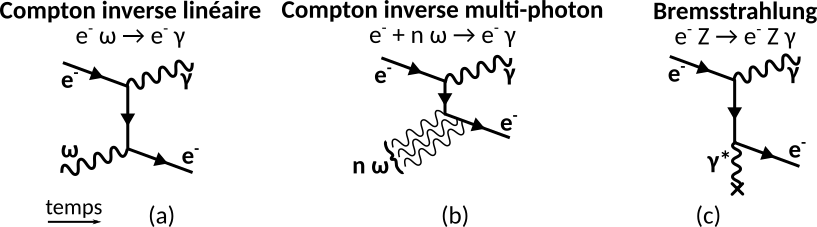
\includegraphics[width=\linewidth]{1-particules/QED_gamma.png}
	\caption{Illustration de processus de production de photons énergétiques par diffusion électron-photon, avec (a) la diffusion Compton inverse dans le régime linéaire, (b) la diffusion Compton inverse dans le régime multi-photon, et (c) le processus Bremsstrahlung, interprété comme la diffusion d'un électron sur un photon virtuel représentant le champ électrique d'une charge électrique.}
	\label{fig:12-diagrammes_gamma}
\end{figure}

Le processus \textbf{Compton inverse linéaire}, représenté sur la figure \ref{fig:12-diagrammes_gamma}a, correspond donc à la \textbf{diffusion inélastique} (i.e. avec transfert d'énergie) \textbf{d'un électron sur un photon réel}. À basse énergie, ce processus est souvent appelé diffusion Thomson, dès lors que le recul de l'électron est faible dans son référentiel propre, soit pour une énergie du photon diffusé $\ll m_e$ dans ce référentiel. On peut aussi noter la similitude entre le diagramme \ref{fig:12-diagrammes_gamma}a, représentant le processus Compton inverse linéaire, et le diagramme \ref{fig:1-diagrammes_electron-positron}a, représentant le processus Breit-Wheeler linéaire, par l'échange d'un électron incident et d'un positron émis, et par l'échange d'un photon émis par un photon absorbé. Dans ce cas, certaines règles de calculs permettent de déduire l'amplitude de transition d'un des processus à partir de l'amplitude de transition de l'autre processus (via le principe de symétrie croisée, ou \textit{crossing symmetry} \parencite{greiner_2009}). La section efficace de ces processus est donc similaire, et de l'ordre de \parencite{carron_2007} $\sigma_{e \omega \to e \gamma} \sim r_e^2$. Néanmoins, comme les particules incidentes et diffusées sont identiques (les particules ne changent pas de type lors du processus), la diffusion Compton inverse ne présente \textbf{pas de seuil en énergie}, contrairement à la création de paires.

Le processus \textbf{Compton inverse multi-photon}, représenté en figure \ref{fig:12-diagrammes_gamma}b, correspond quant à lui à la production d'\textbf{un seul} photon de haute énergie dans la diffusion d'un électron par \textbf{plusieurs} photons de basse énergie. Il peut être rapproché du processus Breit-Wheeler multi-photon, par la même opération que précédemment, et est lui aussi étudié dans le cadre de l'électrodynamique en champ fort. Ce processus a déjà été observé par \cite{bula_1996}, mais présente toujours un fort intérêt théorique \parencite{dipiazza_2012}. 

Enfin, le processus \textbf{Bremsstrahlung} (signifiant "rayonnement de freinage" en Allemand), est représenté en figure \ref{fig:12-diagrammes_gamma}c. Il peut être décrit dans un \textbf{cadre classique}, en considérant le \textbf{rayonnement émis par un électron dévié} (et donc accéléré) \textbf{par le champ électrostatique d'un noyau d'atome} \parencite{jackson_2009}, mais peut aussi être \textbf{interprété de façon quantique comme la diffusion d'un électron sur un photon virtuel} représentant le champ électrostatique associé au noyau \parencite{jackson_2009}. Sa section efficace est de l'ordre de \parencite{carron_2007} $\sigma_{e Z \to e Z \gamma} \sim \alpha Z^2 r_e^2$, et il ne présente pas de seuil en énergie bien que, comme nous le verrons par la suite, la production de photons $\gamma$ par Bremsstrahlung dans la matière est principalement efficace pour des électrons de plusieurs $\si{\MeV}$. Le même processus peut aussi avoir lieu dans le champ électrostatique associé à un électron, avec une section efficace \parencite{carron_2007} $\sigma_{ee\to ee \gamma} \sim \alpha r_e^2$. En négligeant les effets d'écrantage, la section efficace de production de photons dans la diffusion d'un électron par un atome $X$ de numéro atomique $Z$ est donc de l'ordre de $\sigma_{e X \to e X \gamma} \sim \alpha Z(Z+1) r_e^2$, et est largement dominée par la contribution du noyau pour des numéros atomiques élevés \parencite{carron_2007}. Lors de la propagation d'électrons dans la matière, le processus Bremsstrahlung peut être en compétition avec d'autres processus, dont les plus significatifs seront évoqués dans la section suivante.

D'autres processus de production de photons d'énergies autour du MeV sont néanmoins possibles. Par exemple, la déviation d'un électron par un champ magnétique, appelé parfois processus synchrotron ou magnéto-Bremmstrahlung, peut lui aussi être interprété à la fois dans un cadre classique ou en considérant la diffusion d'un électron sur un photon virtuel matérialisant le champ magnétique \parencite{lieu_1993}. Nous pouvons aussi mentionner l'annihilation de particule-antiparticule, ou encore la désexcitation de noyaux atomiques \parencite{diehl_2001}. L'utilisation des niveaux de transitions nucléaires pour produire un laser d'énergie dans la gamme du $\si{\MeV}$ a d'ailleurs été étudié, mais reste pour le moment toujours à démontrer \parencite{rivlin_2007}. De plus, en considérant un faisceau de photons d'énergies largement supérieure au $\si{\MeV}$, le seuil de création de paires peut aussi être atteint par collision avec des photons moins énergétiques. Ces sources de plus basses énergies pourraient alors être produites de multiples façons, et nous verrons au chapitre \ref{chap:3-methodes_exp} que l'utilisation de rayonnement thermique de température de plusieurs centaines d'$\si{\eV}$, ou de photons d'énergies autour du $\si{\keV}$ produits par des laser à rayons X (appelés \textit{XFEL}, pour \textit{X-ray Free Electron Laser}) sont des options étudiées pour la production de paires $e^-e^+$ par le processus BWL.

Dans la suite de ce manuscrit, nous serons intéressés à de nombreuses reprises par la production de photons via le processus \textbf{Bremsstrahlung} lors de la \textbf{propagation d'électrons dans la matière}. Dans ce contexte, ces sources de photons peuvent aussi être significativement affectées par leur propagation dans la matière, en particulier via l'absorption de photons par création de paires au voisinage d'un noyau d'atome (processus Bethe-Heitler). Nous terminerons donc ce chapitre en évoquant très rapidement la phénoménologie de la propagation d'électrons et de photons dans la matière.

\subsection{Propagation d'électrons et de photons dans la matière}

Dans le cadre de cette thèse, nous serons principalement intéressés par des gammes d'énergies de particules typiquement de $10 ~ \si{\keV}$ à $1 ~ \si{\GeV}$. Les processus les plus significatifs pour la propagation des électrons dans la matière sont alors les diffusions élastiques, l'excitation, l'ionisation et Bremsstrahlung, et pour les photons l'effet photo-électrique, la diffusion Compton, la diffusion Rayleigh et la création de paires au voisinage d'une charge électrique (Bethe-Heitler et Triplet). D'autres processus existent néanmoins, mais peuvent être négligés en première approximation pour ces énergies \parencite{carron_2007}.

Lorsque des photons d'énergies $E_\gamma > 2 m_e$ se propagent dans la matière, ceux-ci peuvent produire des paires $e^-e^+$ au voisinage de charges électriques, comme cela a été décrit précédemment. En négligeant les effets d'écrantages, la section efficace de création de paires au voisinage d'un atome $X$ est de l'ordre de $\sigma_{\gamma X \to X e^- e^+} \sim \alpha Z (Z+1) r_e^2$ \parencite{carron_2007}. Celle-ci est alors d'autant plus importante que le numéro atomique du matériau est élevé, et est dans ce cas dominée par le terme en $Z^2$, qui correspond à l'influence spécifique du champ électrique du noyau de l'atome. Ce processus est \textbf{dominant pour des énergies de photons $E_\gamma > 100 ~ \si{\MeV}$ pour tous les matériaux}, et plus précisément à partir de 20 MeV dans l'aluminium ($Z=13$), ou à partir de 5 MeV dans le platine ($Z=78$). À haute énergie, la section efficace de création de paires est quasiment indépendante de l'énergie du photon incident \parencite{carron_2007}. 

Pour des photons d'énergies plus faibles, typiquement \textbf{entre quelques $10$ à $100 ~ \si{\keV}$ et quelques $1$ à $10 ~ \si{\MeV}$}, le processus dominant est la diffusion inélastique de photons sur des électrons libres ou liés, appelée \textbf{diffusion Compton}. C'est le processus inverse de la diffusion électron-photon décrite précédemment, et sa section efficace est donc de l'ordre de $\sigma_{\gamma e \to \gamma e} \sim r_e^2$, pour la diffusion d'un photon sur un électron libre. Pour la diffusion d'un photon sur les électrons liés d'un atome, cette section efficace est de l'ordre de $Z r_e^2$ si on peut négliger l'énergie de liaison de l'électron devant l'énergie du photon incident. C'est le \textbf{processus dominant autour de $1 ~ \si{\MeV}$ pour tous les matériaux}, et la longueur typique d'interaction d'un photon de cette énergie peut être estimée comme étant de l'ordre de $16 \si{[\g\per\cm^2]} / \rho ~ \si{[\g \per \cm^3]})$ où $\rho$ est la masse volumique du matériau \parencite{carron_2007}. Un photon d'énergie autour de $1 ~ \si{\MeV}$ a donc une longueur typique d'interaction autour de $6 ~ \si{\cm}$ dans de l'aluminium ($\rho \sim 2.7 ~ \si{\g \per \cm^3}$), ou autour de $0.8 ~ \si{\cm}$ dans du platine ($\rho \sim 22 ~ \si{\g \per \cm^3}$).

Pour les \textbf{plus basses énergies de photons considérées}, typiquement \textbf{inférieures à quelques $10 ~ \si{\keV}$ à $100 ~ \si{\keV}$}, le processus dominant est l'\textbf{absorption des photons par effet photo-électrique}. Dans l'approximation de Born, sa section efficace pour la couche K a une magnitude proportionnelle \parencite{carron_2007} à $\sigma_K \sim \alpha^4 Z^5 r_e^2$ et est donc \textbf{fortement dépendante du numéro atomique} (cette approximation n'est néanmoins valide que pour des valeurs de $Z$ pas trop élevées \parencite{carron_2007}). Ce processus est dominant pour des énergies de photons $E_\gamma<100 ~ \si{\keV}$ pour $Z<30$, ou pour $E_\gamma<700 ~ \si{\keV}$ pour $Z<90$ typiquement \parencite{carron_2007}. Dans ces gammes d'énergies, les photons peuvent aussi être diffusés de façon élastique, i.e. sans perte d'énergie pour le photon incident. L'effet de ces diffusions est le plus important typiquement autour de $10$ à $100 ~ \si{\keV}$, où la section efficace de diffusion n'excède néanmoins presque jamais plus de $10\%$ de la section efficace des processus dominants à ces énergies (effet photo-électrique et diffusion Compton principalement) \parencite{carron_2007}. 



Comme nous l'avons évoqué précédemment, la production de photons multi-$\si{\MeV}$ dans la matière est principalement causée par le rayonnement de freinage (Bremsstrahlung) d'électrons énergétiques. En négligeant les effets d'écrantages, la section efficace typique de ce processus pour un atome $X$ est de l'ordre de \parencite{carron_2007} $\sigma_{e X \to e X \gamma} \sim \alpha Z(Z+1) r_e^2$, et est dominé par la contribution du champ électrique du noyau (terme en $Z^2$) pour des numéros atomiques élevés. Entre $1$ et $10 ~ \si{\MeV}$, les effets d'écrantage jouent néanmoins un rôle considérable, et le calcul précis de cette section efficace n'est pas si direct \parencite{mangiarotti_2017a}. L'énergie maximale des photons produits est limitée à l'énergie cinétique de l'électron incident, et le nombre de photons est approximativement constant par décade en énergie, impliquant que \textbf{la majorité de l'énergie rayonnée l'est dans des photons d'énergies relativement peu importantes} \parencite{carron_2007}. L'angle et l'énergie typique des photons émis par ce processus sera discuté plus en détail au chapitre \ref{chap:2-laser}. Ce processus est le \textbf{mécanisme de perte d'énergie dominant pour les électrons d'énergies importantes}, d'énergies supérieures à une valeur souvent appelée \textit{énergie critique}. Celle-ci peut être rapidement estimée comme étant de l'ordre de $550 ~ \si{MeV}/Z$ \parencite{deangelis_2018}, pour $12<Z<93$ et avec une précision de l'ordre de $10 \%$. Elle vaut selon cette estimation autour de $40 ~ \si{\MeV}$ pour de l'aluminium ($Z=13$), et autour de $10 ~ \si{\MeV}$ pour du platine ($Z=78$).



Pour des électrons d'énergies inférieures à cette énergie critique, l'ionisation devient le mécanisme de perte d'énergie dominant, même si il est en compétition avec l'excitation. Ces deux processus sont souvent appelés processus \textit{collisionnels}, et leur section efficace est similaire ; de l'ordre de \parencite{carron_2007} $\sigma_{e X \to eX} \sim 4 \pi (\alpha Z^{2/3} r_B)^2$, où $r_B=\hbar/\alpha m_e c \approx 5 \times 10^{-9} ~ \si{\cm}$ est le rayon de Bohr. Cette section efficace est généralement $> 10^{-19} ~ \si{\cm^2}$, et, pour un électron se propageant dans un matériau solide de densité ionique typique $n_i \sim 10^{23} ~ \si{\cm^{-3}}$, \textbf{la distance typique entre deux interactions} (libre parcours moyen) correspondante est donc \textbf{très faible}, généralement $\lesssim 1 ~ \si{\um}$ \parencite{carron_2007}. Pour des électrons incidents d'énergie $\gtrsim ~ \si{\MeV}$, la perte d'énergie est de l'ordre de $10 ~ \si{\eV}$ par collision pour l'excitation, et quelques centaines d'$\si{\eV}$ par collision pour l'ionisation. La \textbf{perte d'énergie par les processus collisionnels} est alors \textbf{souvent traitée comme une perte d'énergie continue} pour ces électrons énergétiques. La diffusion élastique d'un électron sans perte d'énergie est néanmoins possible, avec une section efficace similaire à la section efficace de l'excitation et de l'ionisation \parencite{carron_2007}. De la même manière que précédemment, ces \textbf{diffusions élastiques} sont alors \textbf{très nombreuses} lors du parcours de l'électron dans la matière, et sont souvent appelées \textit{diffusion multiples}. Pour des énergies de plusieurs centaines de $\si{\keV}$, la diffusion élastique est préférentiellement orientée dans la direction de propagation, avec un angle typique de diffusion proportionnel à $1/\gamma_e$, où $\gamma_e$ est le facteur de Lorentz de l'électron \parencite{carron_2007}. À mesure que les électrons perdent de l'énergie, ceux-ci sont donc diffusés avec un angle de plus en plus important, et \textbf{la longueur de parcours totale d'un électron dans la matière est alors supérieure à sa profondeur de pénétration}. Pour un électron d'énergie autour de $1 ~ \si{\MeV}$, cette longueur de parcours est presque indépendante du matériau et vaut autour de $0.6 ~ \si{[\g \per \cm^2]} / \rho ~ \si{[\g \per \cm^3]}$ avec $\rho$ la masse volumique du matériau \parencite{carron_2007}, soit de l'ordre de $0.23 ~ \si{\cm}$ pour de l'aluminium ($\rho \sim 2.7 ~ \si{\g \per \cm^3}$) ou $3.0 \times 10^{-2} ~ \si{\cm} = 300 ~ \si{\um}$ pour du platine ($\rho \sim 22 ~ \si{\g \per \cm^3}$).

Les positrons se comportent quant à eux qualitativement de la même manière que les électrons \parencite{rohrlich_1954}, et sont annihilés préférentiellement à basse énergie \parencite{carron_2007}.


D'un point de vue pratique, la comparaison de ces processus dans de larges gammes d'énergies et de numéros atomiques est souvent menée non pas via des sections efficaces exprimées en $\si{\cm^2}$, mais via une quantité nommée \textit{pouvoir d'arrêt massique}, noté $S_m(E_e)$ et exprimé en $\si{\MeV ~ \cm^2\per\g}$ pour les électrons, et via une quantité nommée \textit{coefficient d'atténuation massique}, noté $\mu_m$ et exprimé en $\si{\cm^2\per\g}$ pour les photons. Ces quantités peuvent alors être comprises comme une \textbf{propriété du matériau} à extraire de l'énergie d'un faisceau d'électrons, ou à atténuer un faisceau de photons. Elles peuvent être reliées aux sections efficaces via les formules \parencite{carron_2007} :
\begin{equation}
    S_m(E_e) ~ \si{[MeV ~ cm^2/g]} = E_e \si{[MeV]} ~\dfrac{\mathcal{N}_A}{A \si{[g/mol]}} ~ \sigma \si{[cm^2]}~ ; ~
    \mu_m \si{[cm^2/g]} = \dfrac{\mathcal{N}_A}{A \si{[g/mol]}} \sigma \si{[cm^2]} ~ \rm ,
\end{equation}
avec $\mathcal{N}_A$ le nombre d'Avogadro et $A$ est la masse atomique du matériau.

Les pouvoirs d'arrêt des électrons et coefficients d'atténuation des photons liés aux différents processus précédemment évoqués sont alors tracés en figure \ref{fig:12-exemples_electrons_photons}, pour l'aluminium ($Z=13$) et le platine ($Z=78$). Ainsi, pour les coefficients d'atténuations affichés en figures \ref{fig:12-exemples_electrons_photons}c et \ref{fig:12-exemples_electrons_photons}d, nous pouvons remarquer que les processus apportant la contribution la plus significative au coefficient d'atténuation massique total sont tour à tour l'effet photo-électrique, la diffusion Compton et la création de paires par Bethe-Heitler, lorsque l'énergie des photons est croissante. Le coefficient d'atténuation massique par création de paires est aussi plus important dans le platine que dans l'aluminium, et ce processus est dominant pour une énergie moins importante dans le matériau de numéro atomique le plus élevé. De la même manière, les processus apportant une contribution dominante au pouvoir d'arrêt massique total sont principalement les processus collisionnels pour les énergies les plus faibles, et le processus radiatif Bremsstrahlung pour les énergies les plus importantes. On peut noter que le pouvoir d'arrêt massique \textit{radiatif}, i.e. faisant intervenir seulement la perte d'énergie par rayonnement, est plus important pour le platine que pour l'aluminium. L'énergie critique de transition entre le régime collisionnel et radiatif est aussi moins importante pour un numéro atomique plus élevé. On peut aussi remarquer que le pouvoir d'arrêt semble croître linéairement avec l'énergie de l'électron incident pour les plus hautes énergies.

\begin{figure}[t]
	\centering
	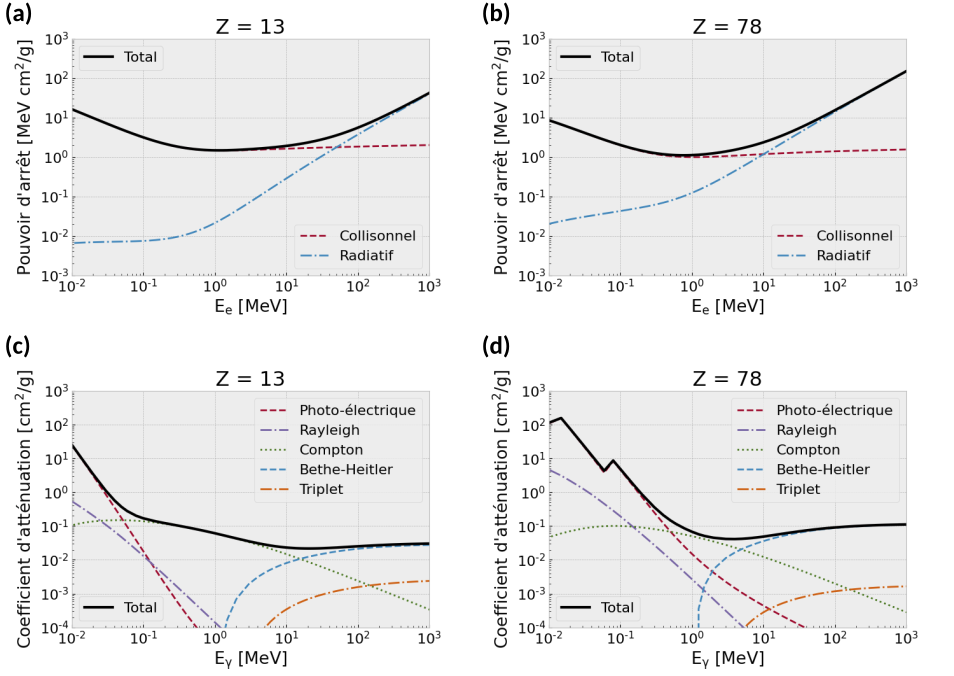
\includegraphics[width=0.9\linewidth]{1-particules/exemples_electrons_photons.png}
    \caption{Exemples de pouvoir d'arrêt des électrons et de coefficient d'atténuation des photons pour respectivement (a) et (c) l'aluminium, ou (b) et (d) le platine. Les données proviennent des bases de données ESTAR et XCOM du NIST \parencite{berger_1999,berger_1999a}, et ont été obtenues à l'aide du module Python \textit{nist-calculators} disponible à l'adresse \href{https://github.com/Zelenyy/nist-calculators}{github.com/Zelenyy/nist-calculators}.}
    \label{fig:12-exemples_electrons_photons}
\end{figure}

Dans ce cadre, ce pouvoir d'arrêt massique est en effet souvent approximé à haute énergie comme \parencite{carron_2007} :
\begin{equation}
    S_m^{rad}(E_e) \approx -\dfrac{E_e}{X_0/\rho}
\end{equation}
où $X_0$ est une longueur caractéristique du matériau nommée \textit{longueur de radiation}, qui peut être estimée par \parencite{carron_2007} :
\begin{equation}
    \dfrac{1}{X_0} = 4 \dfrac{\rho ~ \mathcal{N}_A}{A} \alpha Z (Z+1) r_e^2 \ln\left(\dfrac{183}{Z^{1/3}}\right) ~ \rm .
\end{equation}

La \textbf{perte d'énergie par rayonnement} d'un électron est alors \textbf{plus importante} pour des \textbf{électrons d'énergies importantes}, et pour des \textbf{numéros atomiques élevés}. Selon cette estimation, la longueur de radiation vaut typiquement 11 cm pour de l'aluminium, et 5 mm pour du platine.

Le pouvoir d'arrêt massique total des électrons $S_m$, et le coefficient d'atténuation massique total des photons $\mu_m$ est alors affiché en fonction de l'énergie de la particule incidente et du numéro atomique $Z$ entre $1$ et $100$ respectivement figures \ref{fig:12-processus_matiere}a et  \ref{fig:12-processus_matiere}b.

\begin{figure}[t]
	\centering
	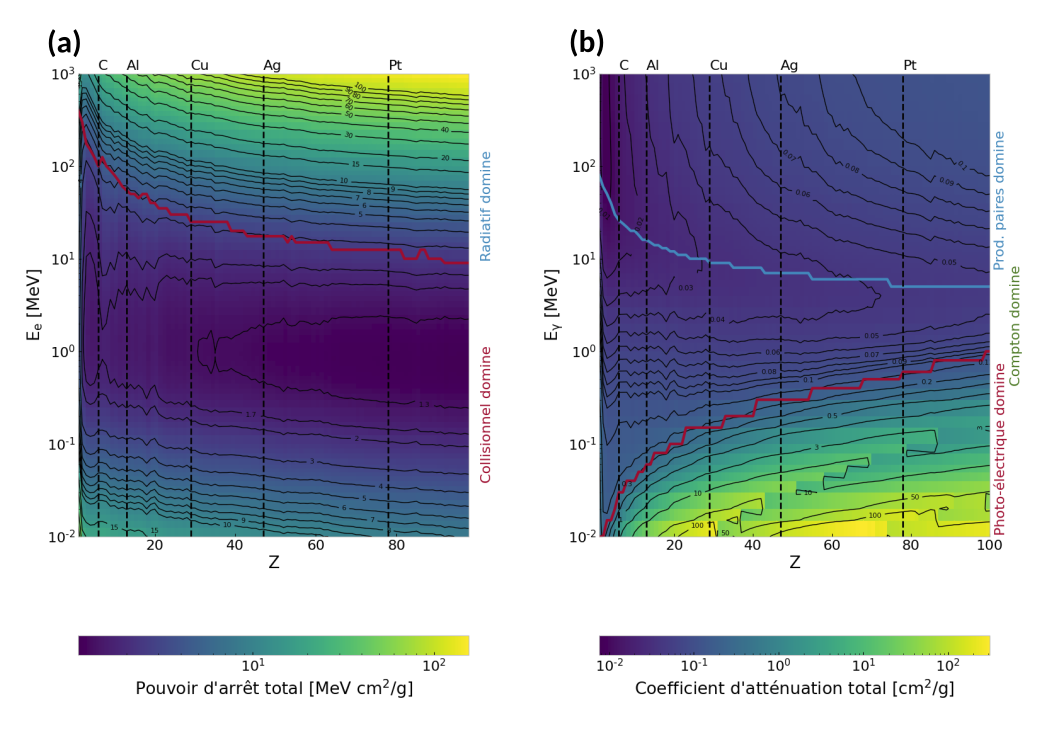
\includegraphics[width=\linewidth]{1-particules/processus_matiere.png}
	\caption{Illustration des processus dominants de l'interaction particule-matière avec (a) le pouvoir d'arrêt massique total des électrons et (b) le coefficient d'atténuation massique total des photons, en fonction de l'énergie des particules incidentes et du numéro atomique. Les données proviennent des bases de données ESTAR et XCOM du NIST \parencite{berger_1999,berger_1999a}, et ont été obtenues à l'aide du module Python \textit{nist-calculators} disponible à l'adresse \href{https://github.com/Zelenyy/nist-calculators}{https://github.com/Zelenyy/nist-calculators}. Cette figure est largement inspirée de \parencite{carron_2007}.}
	\label{fig:12-processus_matiere}
\end{figure}

Ainsi, pour un électron incident de plusieurs dizaines de $\si{\MeV}$ d'énergie, la production de photons est le mécanisme de perte d'énergie dominant, et ce d'autant plus que l'énergie de l'électron incident est importante. Les photons produits avec des énergies multi-$\si{\MeV}$ sont principalement absorbés par création de paires $e^-e^+$ au voisinage de noyaux, ou éventuellement diffusés de façon inélastique. Pour des \textbf{matériaux de numéro atomique élevés}, la \textbf{production de photons est plus efficace} (dépendance en $Z^2$ de la section efficace Bremsstrahlung) mais la \textbf{création de paires dans la matière l'est aussi} (dépendance en $Z^2$ de la section efficace ici aussi). Les \textbf{pouvoirs d'arrêts massiques et les coefficients d'atténuations massique}s étant normalisés par la densité du matériau, ceux-ci ont des \textbf{valeurs proches pour des numéro atomiques proches}. Dans ce cadre, le principal \textbf{effet de la densité} du matériau est de \textbf{concentrer les interactions dans un volume plus faible pour des matériaux plus denses}.


\newpage
\printbibliography[heading=subbibintoc]
\end{refsection}